% nobabel means you'll need to provide your own month names, week day headings,
% etc. We'll use jsarticle+uplatex in this example.
\RequirePackage{scrlfile}
\ReplaceClass{extarticle}{jsarticle}
\AfterClass{jsarticle}{\RequirePackage[20pt]{extsizes}}
\PassOptionsToClass{uplatex}{jsarticle}
\documentclass[giant,nobabel,sundayweek,dvipdfmx]{cdcalendar}

%% and here we do some settings for a calendar in Japanese
\usepackage{jp-mod-uptex}

\usepackage[fleqn]{amsmath}

\usepackage{ebgaramond}
\usepackage[medium]{FiraSans}

\usepackage{graphicx}
\usepackage{fontawesome}
\usepackage{wallpaper}

\graphicspath{{img/}}

%% Define all event mark styles here
\tikzset{holiday/.style={rectangle,fill=orange!70}}
\tikzset{pink icon/.style={text=Pink,font=\large}}
\tikzset{blue icon/.style={text=SkyBlue,font=\large}}

% Default values -- change if needed
% \setlength{\CalPageMargin}{1cm}
% \setlength{\EventLineWidth}{6in}
\geometry{a4paper}

\begin{document}

%%%%%%
% Cover
%%%%%%

\coverBgColor{RoyalBlue!40!black}
\coverImage[\color{gray!50}David R.~Goodsell, RCSB PDB, 2005. `Molecule of the Month 2005 August: Neurotrophins: Receptors for nerve growth factor'. \mbox{CC-BY-4.0.} \url{https://doi.org/10.2210/rcsb_pdb/mom_2005_8}]
{68-Neurotrophins-receptors}

\coverTitle[font=\fontsize{56pt}{56pt}\sffamily\bfseries\gtfamily,
text=white,text width=\linewidth,align=flush right]
{2019カレンダー}

\makeCover

% Remove this line if you feel the background pattern is too annoying
% \TileWallPaper{.5\paperwidth}{.5\paperheight}{ricepaper_v3}
\TileWallPaper{.5\paperwidth}{.1\paperheight}{lightpaperfibers}

%%%% Remove this page if you don't need it --
%%%% just to show the actual output
% {\centering
% 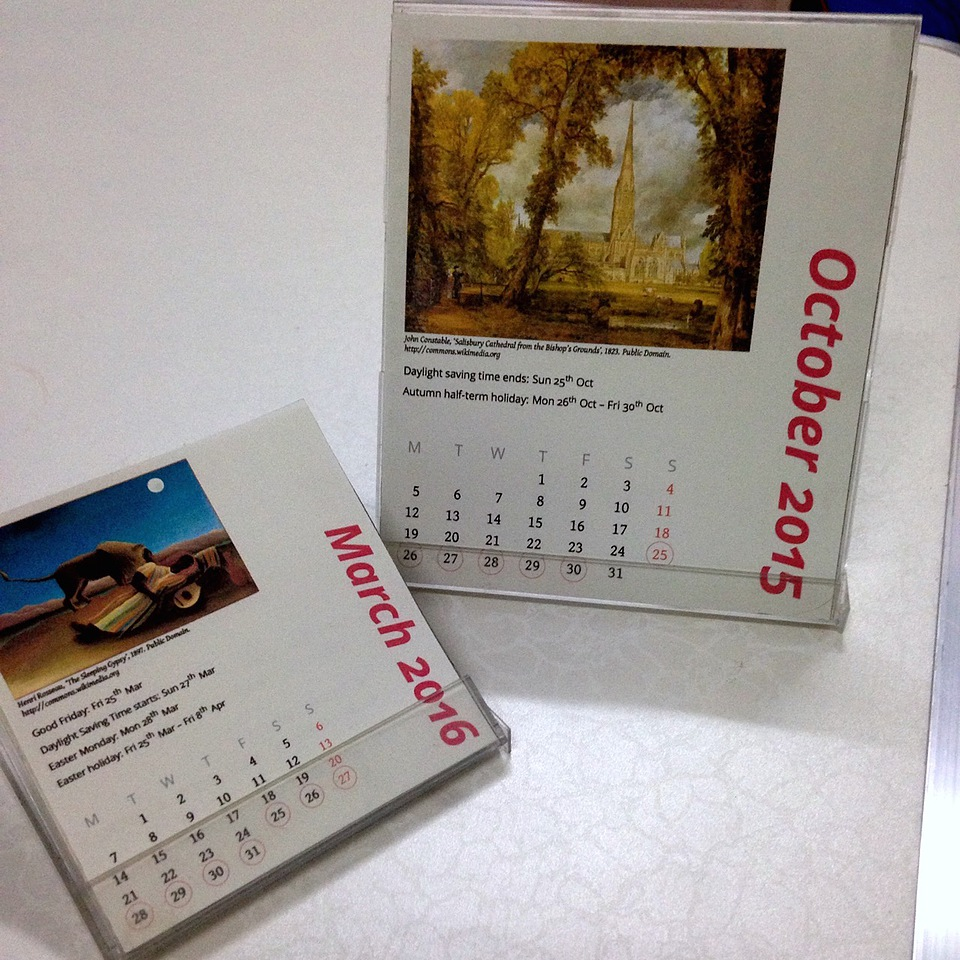
\includegraphics[width=\textwidth]{actual}
% \par}

% {\small ここに実際に印刷されたカレンダーがあります。 小さなカレンダー(9\,cm $\times$ 9.5\,cm)は、フロッピーディスクのジュエルケースに適合します。 大きなもの(11.7\,cm $\times$ 13.65\,cm)はCDのジュエルケースに適合します。\par}

% \clearpage
%%%%

% You may find the gap between illustrations and events too narrow
% Use this length to increase it
\setlength{\illusSkip}{1em}


%%%%%%
% Some settings for the monthly calendars
%%%%%%
\dayHeadingStyle{font=\gtfamily\color{gray!90}}
\sundayColor{red}
\monthTitleStyle{font={\fontsize{42pt}{44pt}\gtfamily\sffamily}, red!50!RedViolet}
\eventStyle{\scriptsize\sffamily\gtfamily}

%%%%%%
% January 2019
%%%%%%
\illustration
[`Detail of a power 20 mandelbulb made using Visions of Chaos'. By Soler97—Own work, Public Domain. \url{http://bit.ly/2hcn1gM}]
{\linewidth}{Mandelbulb140a}


\begin{monthCalendar}{2019}{01}


%%% events must be given AFTER \begin{monthCalendar}
%%% Currently you must give events on the same page
%%% as the monthly calendar.

%% This is a two-day event
\event[mark style=holiday]{2019-01-01}{2}{元日 振替休日}
%% or you can write \event{2019-01-01}{2019-01-02}{元日 振替休日}

%% This is an one-day event
\event[mark style=blue icon, marker=\faBlackTie]
{2019-01-09}{}{成人の日}

%% This is a 5-day event
\event[mark style=blue icon,marker=\faBriefcase]{2019-01-30}{5}{ACME会議}
%% you could also write \event{2019-01-06}{2019-02-03}{ACME会議}
\end{monthCalendar}

\clearpage

%%%%%%
% Feb 2019
%%%%%%

% Or you can put any stuff, really, with a caption if you want:
\setlength{\mathindent}{0pt}
\otherstuff[Legrange's Equation, one of the `greatest mathematical equations'. \url{http://www.livescience.com/26680-greatest-mathematical-equations.html}]
{\linewidth}
{\huge\selectfont\[%
  \frac{d}{dt}\left(\frac{\partial \textcolor{red}{L}}{\partial \dot{q}_i}\right) = \frac{\partial \textcolor{red}{L}}{\partial q_i}
\]}

\begin{monthCalendar}{2019}{02}

%% Repeat the event if it spans two months
\event[mark style=blue icon,marker=\faBriefcase]{2019-01-30}{5}{ACME会議}
\event[mark style=pink icon,marker=\faBirthdayCake]{2019-02-14}{}{友人の誕生日}
\event{2019-02-22}{}{締め切り!}

\end{monthCalendar}

\end{document}
